\documentclass{article}

\usepackage[utf8]{inputenc}
\usepackage{amsmath}
\usepackage{amssymb}
\usepackage{hyperref}
\usepackage{multirow}
\usepackage[most]{tcolorbox}
\tcbuselibrary{skins,breakable}

\newtcolorbox{callout}[2][]{breakable,sharp corners, skin=enhancedmiddle jigsaw,parbox=false,
boxrule=0mm,leftrule=2mm,boxsep=0mm,arc=0mm,outer arc=0mm,attach title to upper,
after title={.\ }, coltitle=purple,colback=purple!10,colframe=purple, title={#2},
fonttitle=\bfseries,#1}

\newtcolorbox{warning}[2][]{breakable,sharp corners, skin=enhancedmiddle jigsaw,parbox=false,
boxrule=0mm,leftrule=2mm,boxsep=0mm,arc=0mm,outer arc=0mm,attach title to upper,
after title={!\ }, coltitle=red,colback=red!10,colframe=red, title={#2},
fonttitle=\bfseries,#1}

\newtcolorbox{esempio}[2][]{breakable,sharp corners, skin=enhancedmiddle jigsaw,parbox=false,
boxrule=0mm,leftrule=2mm,boxsep=0mm,arc=0mm,outer arc=0mm,attach title to upper,
after title={:\ }, coltitle=blue,colback=blue!10,colframe=blue, title={#2},
fonttitle=\bfseries,#1}

\newcommand{\na}[0]{\ensuremath {\overset{N}{\rightarrow}}}
\newcommand{\rl}[3]{\inference{#1}{#2}\text{ #3}}
\newcommand{\bop}[0]{\ensuremath\oplus}
\newcommand{\appl}[2]{\ensuremath(#1)\ #2}
\newcommand{\st}[3][]{\ensuremath{\displaystyle\frac{#3\hfill}{#2\hfill} \text{#1}}}
\newcommand{\N}{\ensuremath \mathbb N}
\newcommand{\I}{\ensuremath \mathbb I}
\newcommand{\lam}[2]{\ensuremath{\lambda#1.#2}}
\newcommand{\inl}[0]{\ensuremath{\ inl\ }}
\newcommand{\inr}[0]{\ensuremath{\ inr\ }}
\newcommand{\case}[3]{\ensuremath{\text{case}#1\ \text{of}\ \left|\begin{aligned}& #2\\ & #3\end{aligned}\right.}}
\newcommand{\Da}[0]{\ensuremath{\Downarrow}}
\newcommand{\while}[2]{\ensuremath{\text{while }#1\text{ do }#2\text{ end}}}
\newcommand{\for}[3]{\ensuremath{\text{for }i=#1\text{ to }#2\text{ do }#3\text{ end}}}
\newcommand{\mE}[0]{\ensuremath{\mathbb{E}}}
\newcommand{\pair}[1]{\ensuremath{\langle#1\rangle}}
\newcommand{\V}{\ensuremath{\mathcal{V}}}
\newcommand{\cE}{\ensuremath{\mathcal{E}}}
\newcommand{\cD}{\ensuremath{\mathcal{D}}}
\newcommand{\cF}{\ensuremath{\mathcal{F}}}
\newcommand{\IF}[0]{\ensuremath {\text{ if }}}
\newcommand{\THEN}[0]{\ensuremath {\text{ then }}}
\newcommand{\ELSE}[0]{\ensuremath {\text{ else }}}
\newcommand{\AND}[0]{\ensuremath {\text{ and }}}
\newcommand{\OR}[0]{\ensuremath {\text{ or }}}
\newcommand{\unpack}[3]{\ensuremath{\text{unpack } #1 \text{ as }\langle #2 \rangle\text{ in }#3}}
\newcommand{\pack}[2]{\ensuremath{\text{pack } \pair{#1} \text{ as } #2 }}
\newcommand{\te}[1]{\text{#1}}
\newcommand{\ls}[0]{\ensuremath{\leadsto^{*}}}
\newcommand{\LET}[0]{\ensuremath{\text{ let }}}
\newcommand{\TIN}[0]{\ensuremath{\text{ in }}}
\newcommand{\NEW}[0]{\ensuremath{\text{ new }}}

\usepackage[parfill]{parskip}

\title{Computer Vision}
\author{Diego Oniarti}
\date{Anno 2024-2025}

\begin{document}

\maketitle
\tableofcontents

\newpage
\section{24-02-2025}
\subsection*{Main topics of the course}
\begin{enumerate}
    \item acquisition
    \item motion detection
    \item motion analysis
    \item stereo/multi -view
    \item 3D point cloud
    \item feature extraction / classification
\end{enumerate}

\subsection*{Evaluation}
The written exam will be 40\% of the vote.\\
You can choose between a project and an oral exam. If you're not satisfied with the result of the written you can take an oral later.

Reading groups are also a thing.

\begin{itemize}
    \item 24 mar: teams + project ideas
    \item 31 mar project titles assignment for those who haven't chosen one
\end{itemize}

For the project we'll use python, openCV, and ffmpeg.

You can deliver the project and written exam in different sessions. But the written exam expires in 1 year.

\newpage
\section{28-02-2025}
\subsection*{Bayer Pattern} is a pattern used in camera sensors to optimize the distribution of colors. Since the human eye is more sensitive to green light, the pattern is composed of a checkerboard pattern where one color is green and the other is divided between red and blue.

\subsection*{Quantization} Usually we use 8bpp (bits per pixel) because it is byte aligned and because it's plenty enough for the human eye. At lower bpp, contouring appears.

\subsection*{Video} Static images loose the temporal and movement information, so we need videos.\\
The frame rate of an image must be compliant with the thing that is being captured. With an high enough rate we can ensure a smooth transition between frames without loosing information.

This is the reason video-cameras usually have a lower resolution that photo-cameras. With too high of a resolution, there is too much information that needs to be processed and it can't be done at a fast enough rate.

Humans also focus less on image quality while watching a video, as they're more captivated by the evolution of events than the single frames.

\subsection*{Relevant features} The relevant features in an image are color, edges, and contrast.
In a video the features are the same but also their progression through time.

\subsection*{Image compression} Image take up a lot of space and videos take up even more. Compression standards exist to reduce the amount of data required.\\
Compression requires there to be an \textbf{encoder} and a \textbf{decoder}. Some examples are JPEG, MPEG, and DIVX.
Both visualization and processing are executed on the uncompressed image, since humans can't visualize raw compressed data, and filters can't work on the compressed image.

Some compression algorithms are lossy while some other are lossless.

\subsection*{Histogram} is a simple way to describe the color distribution of a picture by approximating a probability function.
\begin{align*}
    hist(p) = \frac{\# pixels: I(x,y)=p}{N\cdot M} \approx f(p)
\end{align*}
Where $N,M$ are the size of the picture in pixels.

Various filters can be applied to an image by manipulating the histogram with operations like stretching and thresholding.

We can equalize an histogram defining a partial sum $CHist_I(p) = \sum_{k=0}^p hist(k)$ e assegnando $hist_{eq}(p) = \frac{CHist(p) - CHist_{min}}{M\cdot N -1} \cdot 255$.\\
Even equalizing we can not get to a flat histogram, but we can do our best to get to that point.

\subsection*{Edge extraction} Usual Sobel su X, Y, thresholding, etc. Convolution in 1D and its natural translation in two dimensions.\\
A convolution in the space domain is equivalent to a product in the frequency domain and vice versa.

\subsection*{Low-pass filtering}
The easiest way to implement a discrete low pass filter is to design a kernel that takes the average of the values surrounding a pixel.\\
A better visual result is given by a Gaussian filter. Funnily enough, the Fourier transform of a gaussian curve is still a gaussian curve.

\subsection*{Low Pass vs Median}
Low pass filtering can reduce noise in an image, but it also spreads the noise over the image. In some cases this may be undesirable. The common approach would be to threshold the filtered image, but finding the threshold value can be cumbersome.

Some other filters to denoise is the \textbf{median filter}. It's not \textit{isotropic} and it doesn't work with a normal convolution, but it requires a \textit{sorting} operator.

Gaussian and averaging filters introduce in the image values that were not in the original image. The median filter, instead, only "selects" values from the image, not inventing new ones.

\section{Morphology}
A form of non linear filtering that refers to the shape of a region.

Goals:
\begin{itemize}
    \item check whether a certain shape fits into another
    \item check whether a picture has holes of a certain size
    \item remove areas smaller than a threshold
\end{itemize}

\section*{Binary morphology}
We need a \textbf{binary image}\footnote{A binary image is not grayscale but an image composed only of true and false} and \textbf{structuring elements} and implement four main operations:
\begin{itemize}
    \item erosion
    \item dilation
    \item opening
    \item closing
\end{itemize}
Erosion and dilation are intuitive, enlarging or reducing the size of a region. Opening and closing are combinations of erosion and dilation in sequence.

Structuring elements can be squares, circles, other primitives, or custom shapes. For every structuring element we need to define a "center". It is usually the geometric center of the image but it doesn't have to be.

\subsection{Dilation}
Dilation performs an $\oplus$ (or) operation between the image and the element. More specifically:
\begin{itemize}
    \item sweep the element over the image
    \item if the origin of the element touches the image (a $1$ in the image).
        \begin{itemize}
            \item perform the or, "stamping" the element onto the image
        \end{itemize}
\end{itemize}
It is important to note that the output of the filter has to be stored in a separate image, to avoid it recursively dilating a pixel across the whole image.

\subsection{Erosion}
Erosion works in a similar way by scanning the element over the image:
We don't check with the center of the element anymore but we "activate" the filter when every $1$ in the filter overlaps a $1$ in the image.\\

Question: In the output image, do we only put the center of the element or the whole element?

\subsection{Closing and Opening}
Closing: dilate and then erode \\
Opening: erode and then dilate.

Closing fills the holes in the image with the dilation, and then removes the excess added by the first operation with erosion.\\
Similar but inverse result is gotten by opening. The holes are enlarged, eating away at the shape. Then the remaining bits are consolidated.

\section{Models}
\subsection{Pinhole camera model}
It consists of a box with a small hole on one of the walls. The light that passes through that hole projects a reflected image of the outside world onto the opposite wall.\\
One clear problem is that only a small amount of light can pass through the hole, making the projection very dim. We can fix this by making the hole bigger but this also makes the image blurry.

If the \textit{image plane} is the plane opposite to the camera, the \textit{virtual image plane} is an imaginary plane parallel to the image plane and equally spaced with the pinhole in the other direction.

\paragraph{Model to reality} How do we map the pixel location to a location in space? Following the pinhole camera model we would also need the focal length $f$ of the camera.\\
Then we know the point in space is somewhere on the line that passes through the pixel and the origin shifted by the focal length.
\begin{center}
    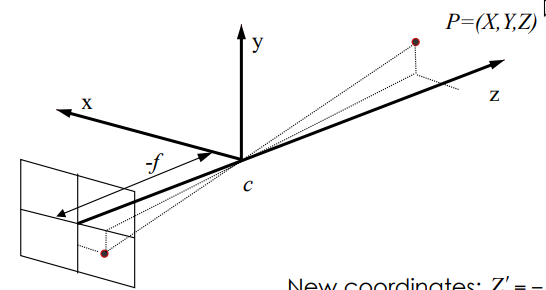
\includegraphics[width=0.8\linewidth]{images/focal.png}
\end{center}
\begin{align*}
    \begin{array}{cc}
        \te{new coordinates} & \te{From the camera}\\
        \begin{cases}
            Z' = -f \\
            X' = -f\frac{X}{Z} \\
            Y' = -f\frac YZ
        \end{cases} 
                             &
        (X,Y,Z) \to (x,y,f) = (f\frac XZ, f\frac YZ, f)
    \end{array}
\end{align*}

It's easy to see that we loose some information, since a point in the camera plane is mapped to a whole line in the real world, loosing the distance.\\
We can approximate the distance with context clues, knowing additional information about the space etc. but these are not means of \textbf{measuring} the distance, only approximating it.

\paragraph{Multiple cameras} To solve the problem of the loss of information we can use \textit{two cameras}, or even more, to measure depth.

Properties of the pinhole model
\begin{itemize}
    \item Parallel lines converge to a single vanishing point
    \item Parallel lines on the same plane lead to collinear vanishing points
    \item The line is called the horizon for a plane
    \item Vertical lines are perpendicular to the horizon
\end{itemize}

\subsection{Orthographic projection model}
The \textit{orthographic projection model} assumes that all rays originated from the 3D object and from the scene are parallel among each other.
The image plane is parallel to $(X, Y)$

Mathematically we're just taking the $x$ and $y$ of the point we're capturing, completely disregarding the depth component. This works since the model assumes object behave the same way regardless of distance.
\begin{align*}
    \left[
    \begin{array}{c}
        x\\ y
    \end{array}
\right] 
    = 
    \left[
    \begin{array}{ccc}
        1 &0&0\\0&1&0
    \end{array}
\right] 
    \left[
    \begin{array}{c}
        X\\ Y\\ Z
    \end{array}
\right] 
\end{align*}

\section{Illumination models}
Illumination is an important component in understanding the content of an image. Different lighting can change the colors perceived in the image, change the shape of perceived edges, etc.

Some materials and surfaces respond to light in different manners, depending how much they \textbf{absorb}, \textbf{reflect}, and \textbf{transmit} it.

Reflections can be
\begin{itemize}
    \item Specular: more energy is concentrated in the light source direction
    \item Diffuse: constant in all directions
\end{itemize}
Surfaces vary in \textit{specularity}, going from matte to glossy. Glossy materials are harder to work with, because they introduce things in the image that are not "real".

\paragraph{Illumination from one light source}
Problem: determine how the surface is irradiated by the light source
assumption: light is far, we can assume all rays can be represented by a single unit vector $s$ (ortho projection)

For each surface element the light is irradiated considering the cosine of the angle between the surface normal and the light direction

\subsection{Lambertian surface}
Model for diffuse reflection, so the specular reflections are ignored. It is possible to make this assumption when the surface is rough enough.

The luminance of a surface in this model is the same regardless of the viewing angle.

This model assumes every surface has a property $\rho$ (\textit{albedo}) that describes how much of the light is reflected by the object.


\end{document}
